\chapter{Matematik Opgaver}

\section*{Differentialregning}
\begin{opgave}{Afledte og dobbeltafledte}{1}
Find den afledte og dobbeltafledte med hensyn til $x$ for følgende funktioner:
\opg $f(x) = x^3$
\opg $f(x) = x^2 + 4x$
\opg $f(x) = \frac{1}{x} + \frac{1}{x^2}$
\opg $f(x) = \cos x$
\opg $f(x) = \ln x$
\end{opgave}

\begin{opgave}{Sammensatte funktioner}{1}
Skriv følgende udtryk som en sammensat funktion ($f(g(x)$). (Altså skal du identificere den indre funktion $g(x)$ og den ydre funktion $f(g)$). Udregn herefter $\d{f}{x}$. 
\opg $f(x) = \sin (4x)$
\opg $f(x) = \sqrt{2x}$
\opg $f(x) = \sqrt{4x+5}$
\opg $f(x) = \sin(e^x)$
\end{opgave}

\begin{opgave}{$f$ som funktion af $g$}{1}
	Udtryk $\d{f}{x}$ vha. den ukendte funktion $g(x)$ og dens
	differentierede $\d{g}{x}$ for følgende funktioner:
	\opg $f(x) = x^2 g(x)$
	\opg $f(x) = \left(g(x)\right)^2$
	\opg $f(x) = g(x^2)$
\end{opgave}

\begin{opgave}{Hastighed og postion}{1}
\begin{figure}[h!]
  \centering
  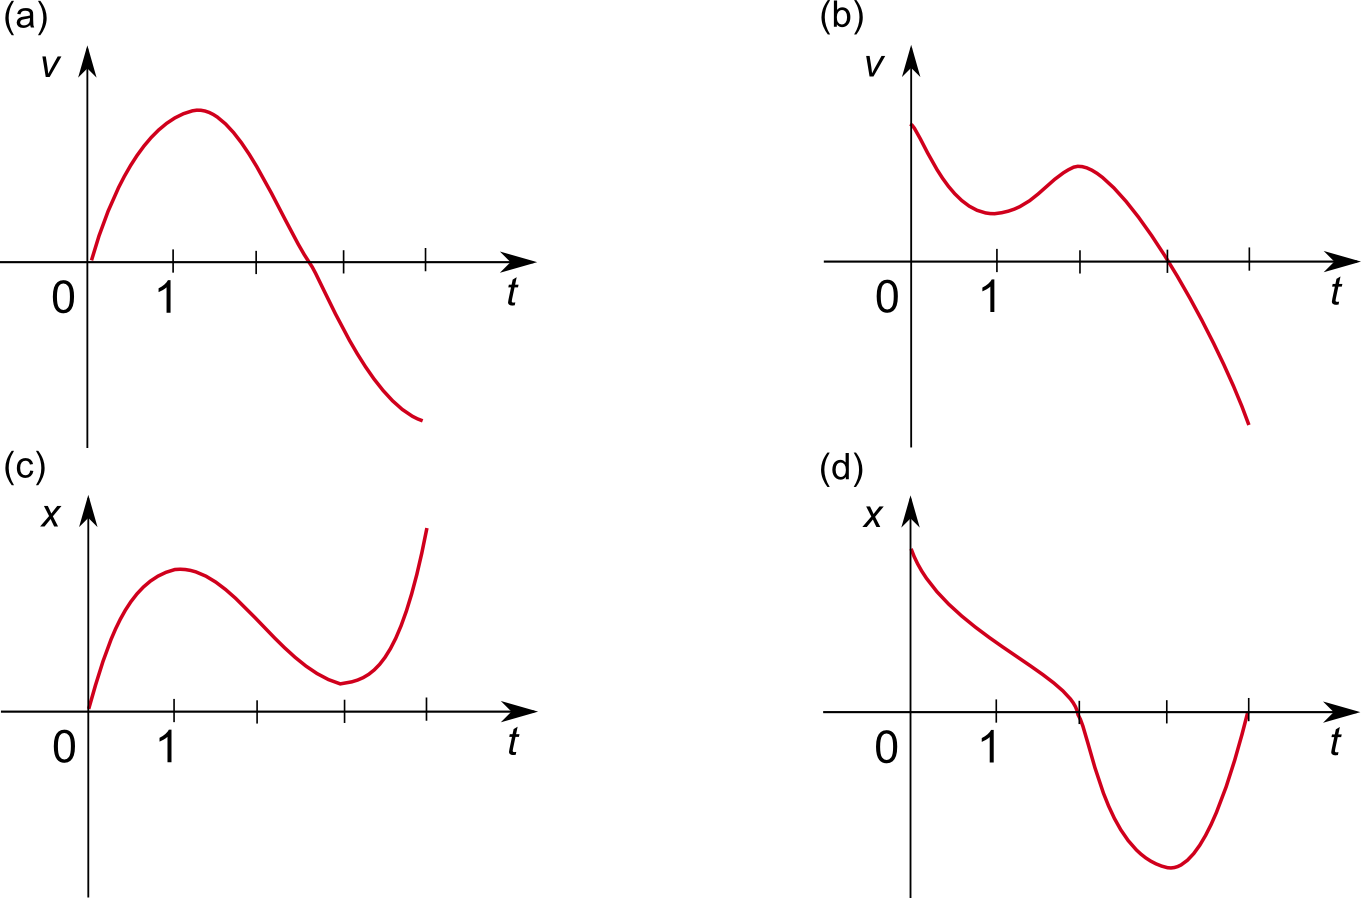
\includegraphics[width=0.6\textwidth]{matematik/vx_grafer.png}
  \caption{Hastighed og position som funktion af tiden.}
  \label{fig:vx_grafer}
\end{figure}
\opg Figur \ref{fig:vx_grafer} (a) og (b) viser farten af to objekter som funktion af tiden i sekunder. Hvornår sætter de to objekter farten op og hvornår sætter de farten ned? Forklar dit svar.
\opg Figur \ref{fig:vx_grafer} (c) og (d) viser positionen af to objekter $x$ som funktion af tiden i sekunder. Hvornår sætter de to objekter farten op og hvornår sætter de farten ned? Forklar dit svar.
\end{opgave}

\begin{opgave}{Harmonisk bevægelse}{2}
Hvis bevægelsen for et objekt er beskrevet vha. positionen
\begin{equation*}
x = A \cos (\omega t + \phi),
\end{equation*}
hvor $A$, $\omega$ og $\phi$ er konstanter, så siger man, at objektet undergår \emph{simpel harmonisk bevægelse}. 
\opg Hvad er hastigheden af objektet til tiden $t$ (som funktion af $t$)?
\opg Hvornår er hastigheden 0?
\end{opgave}

\begin{opgave}{Cepheide-stjernen Delta Cephei}{2}
En Cepheide-stjerne er en bestemt type stjerne, hvis lysstyrke varierer periodisk. En bestemt Cepheide-stjerne har tiden 5,4 dage mellem hver maksimal lysstyrke. Den gennemsnitlige lysstyrke af stjernen er 4,0 med en ændring i lys på $\pm$ 0,35. Hvis $t$ måles i dage, så kan lysstyrken $B$ af denne Cephide-stjerne modelleres af følgende udtryk:
\begin{equation*}
B(t) = 4,0 + 0,35\sin \left( \frac{2\pi t}{5,4} \right).
\end{equation*}
\opg Hvad er raten for ændringen af lysstyrken (ændring af lysstyrke over ændring af tid) som funktion af antal dage $t$?
\opg Hvor meget har lysstyrken ændret sig efter to dage?
\end{opgave}

\begin{opgave}{Udvidelse af ballon}{2}
Der pumpes luft ind i en sfærisk ballon. Til enhver tid $t$ er volumet af ballonen $V(t)$, mens radius af ballonen er $r(t)$.
\opg Hvad er betydningen af de afledte $\d{V}{r}$ og $\d{V}{t}$?
\opg Udtryk $\d{V}{t}$ som funktion af $\dt{r} = \d{r}{t}$.
\end{opgave}

\begin{opgave}{Approksimation af funktion}{3}
  En vilkårlig funktion $f(x)$ kan muligvis være kompliceret, men i
  fysik er vi ofte kun interesseret i, hvordan $f(x)$ i et bestemt
  område af $x$-værdier, f.eks. når $x$ er lille. Heldigvis findes der
  en metode til at approksimere en funktion $f(x)$ omkring et bestemt
  punkt $a$. Når $x \approx a$ kan vi approksimere funktionen $f(x)$
  som:
  \[
  f(x) = f(a) + (x-a) \left.\d{f}{x}\right|_{x=a}
  + \tfrac{1}{2} (x-a)^2 \left.\dd{f}{x}\right|_{x=a}
  + \tfrac{1}{3!} (x-a)^3 \left.\frac{d^3f}{dx^3}\right|_{x=a}
  + \ldots
  \]
  Jo flere led, man tager med i summen, jo bedre bliver
  approksimationen af $f(x)$. Ofte er det nok at tage de første 2
  eller 3 led med for at få en god beskrivelse af $f(x)$ for $x
  \approx a$.
  \opg Diskuter betydningen af de enkelte led i summen. Hvordan ser de
  ud som funktioner af $x$, og hvorfor bliver approksimationen bedre
  af at tage flere led med?
  \opg Vis, at når $x \approx 0$, er $\sin x \approx x$ og $\cos x
  \approx 1$ ved kun at medtage de to første led i summen. Hvad bliver
  approksimationerne for $\sin x$ og $\cos x$, hvis du også medtager det
  tredje led?
  \opg Vis, at når $x \approx 1$, er $\ln x \approx x -
  \tfrac{1}{2} x^2$.
  \opg Vis, at når $x \approx 0$, er $e^x \approx 1 + x + \tfrac{1}{2}
  x^2$.
  \opg Vis, at når $x \approx 0$, er approksimationen for et polynomie
  $a_0 + a_1 x + a_2 x^2 + \ldots$ givet ved leddene i polynomiet
  selv. Prøv evt. at beregne de enkelte led i approksimationen for et
  andengradspolynomie.
  \opg Vis, at når $x \approx 0$, er $(1 + x)^a \approx 1 + ax$.
\end{opgave}

\section*{Differentialligninger}

\begin{opgave}{Specialtilfælde af 1. og 2. Ordens Differentialligninger}{1}
I denne opgave skal I vise, at nogle forskellige funktioner er løsninger til de givne differentialligninger.
\opg Vis at funktionen $f(t) = -7e^{3t}$ løser differentialligningen $\d{f}{t} = 3 f(t)$.
\opg Vis at funktionen $g(t) = \frac{2}{3}e^t + e^{-2t}$ løser differentialligningen $\d{g}{t} +2g(t) = 2e^t$.
\opg Vis at funktionen $h(t) = 5 \sin (3t) - 10 \cos(3t)$ løser differentialligningen $\dd{h}{t} = -9h(t)$.
\opg Tjek om funktionen $k(t) = 13 \cos (8t + 45)$ løser differentialligningen $\dd{k}{t} = -64k(t)$.
\end{opgave}

\begin{opgave}{Generelle 1. Ordens Differentialligninger.}{2}
I denne opgave skal I også vise, at nogle forskellige funktioner er løsninger til de givne differentialligninger. Denne gang er funktionerne og differentialligningerne dog skrevet op på en mere generel form, dvs. at de kan indeholde arbitrære konstanter.
\opg Vis at alle funktioner på formen $h(x) = 1 / \left( x + A \right)$ løser differentialligningen $\d{h}{x} = - h(x)^2$.
\opg Vil at alle funktioner på formen $k(x) = \left( c - x^2 \right)^{-1/2}$ løser differentialligningen $\d{k}{x} = x k(x)^3$.
\opg Vis at alle funktioner på formen $g(x) = \left( \ln x + C \right) / x$ løser differentialligningen $x^2 \d{g}{x} + xg(x) = 1$. 
\opg Vis at alle funktioner på formen $f(x) = (1 + ce^x) / (1-ce^x)$ løser differentialligningen $\d{f}{x} = \frac{1}{2} \left( f(x)^2 - 1 \right)$. 
\end{opgave}

\begin{opgave}{Hvornår er det en løsning?}{3}
I denne opgave skal I finde ud af, hvornår nogle forskellige funktioner er løsninger til de givne differentialligninger. Sagt med andre ord skal I finde de specifikke værdier for nogle af de konstanter, der indgår i funktionerne, som gør at funktionerne løser differentialligningerne.
\opg For hvilke værdier af $k$ løser funktionen $f(y) = \cos (ky)$ differentialligningen $4 \dd{f}{y} = - 25f(y)$?
\opg Tjek for de værdier af $k$ I fandt i 1), at funktionen $g(y) = A \sin (ky) + B \cos (ky)$ også løser differentialligningen $4 \dd{g}{y} = -25 g(y)$ (hint: vent med at indsætte værdierne af $k$ før til sidst).
\opg For hvilke værdier af $r$ løser funktionen $h(y) = e^{ry}$ differentialligningen $2 \dd{h}{y} + \d{h}{y} - h(y) = 0$?
\opg Lad $r_1$ og $r_2$ være de konstanter du fandt i 3). Tjek at funktionen $k (y) = ae^{r_1y} + be^{r_2y} $ også løser differentialligningen $2 \dd{k}{y} + \d{k}{y} - k(y) = 0$ (hint: vent med at indsætte værdierne af $r_1,r_2$ før til sidst).
\end{opgave}


\newpage

\chapter{Matematik Facitliste}
\section*{Differentialregning}
\begin{opgave}{Afledte og dobbeltafledte}{1}
\opg $f(x) = x^3$: 
\begin{equation*}
\d{f}{x}=3x^2,~~ \dd{f}{x}=6x
\end{equation*}
\opg $f(x) = x^2 + 4x$:
\begin{equation*}
\d{f}{x}=2x+4,~~ \dd{f}{x}=2
\end{equation*}
\opg $f(x) = \frac{1}{x} + \frac{1}{x^2}=x^{-1}+x^{-2}$: 
\begin{equation*}
\d{f}{x} = - x^{-2}-2x^{-3}, ~~\dd{f}{x}=2x^{-3}+6x^{-4}
\end{equation*}
\opg $f(x) = \cos x$: 
\begin{equation*}
\d{f}{x}= - \sin x,~~ \dd{f}{x}=-\cos x
\end{equation*}
\opg $f(x) = \ln x$: 
\begin{equation*}
\d{f}{x}= \frac{1}{x}=x^{-1},~~\dd{f}{x}=-x^{-2}
\end{equation*}
\end{opgave}

\begin{opgave}{Sammensatte funktioner}{1}
$g(x)$ og $f(g)$ findes. $\d{f}{x}$ findes vha. kædereglen: $\d{f}{x} = \d{g}{x} \cdot \d{f}{g}$.
\opg $f(x) = \sin (4x)$:
\begin{align*}
g(x) &= 4x, ~~f(g)=\sin(g) \\
\rightarrow &\d{f}{x} = 4\cos(4x)
\end{align*}
\opg $f(x) = \sqrt{2x}$:
\begin{align*}
g(x) = 2x, ~~ f(g)=\sqrt{g} \\
\rightarrow \d{f}{x} = 2\frac{1}{2\sqrt{2x}}=\frac{1}{\sqrt{2x}}
\end{align*}
\opg $f(x) = \sqrt{4x+5}$
\begin{align*}
g(x) = 4x+5, ~~f(g)=\sqrt{g} \\
\rightarrow \d{f}{x} = 4\frac{1}{2\sqrt{4x+5}}=\frac{2}{\sqrt{4x+5}}
\end{align*}
\opg $f(x) = \sin(e^x)$
\begin{align*}
g(x) = e^x, ~~f(g)=\sin(g) \\
\rightarrow \d{f}{x} = e^x \cos(e^x)
\end{align*}
\end{opgave}


\begin{opgave}{$f$ som funktion af $g$}{1}
Udtryk $\d{f}{x}$ vha. den ukendte funktion $g(x)$ og dens
differentierede $\d{g}{x}$ for følgende funktioner:
\opg $f(x) = x^2 g(x)$. Produktreglen anvendes:
\begin{equation*}
\d{f}{x} = \d{x^2}{x}\cdot g(x) + x^2\d{g}{x} = 2xg(x)+x^2 \d{g}{x}
\end{equation*}
\opg $f(x) = \left(g(x)\right)^2$. Produktreglen anvendes:
\begin{equation*}
\d{f}{x} = \d{g}{x} g(x) + g(x)\d{g}{x} = 2g(x)\d{g}{x}
\end{equation*}
\opg $f(x) = g(x^2)$. Kædereglen anvendes:
\begin{equation*}
\d{f}{x}=2x\d{g}{x^2}
\end{equation*}
\end{opgave}
\begin{opgave}{Hastighed og postion}{1}
\begin{figure}[h!]
  \centering
  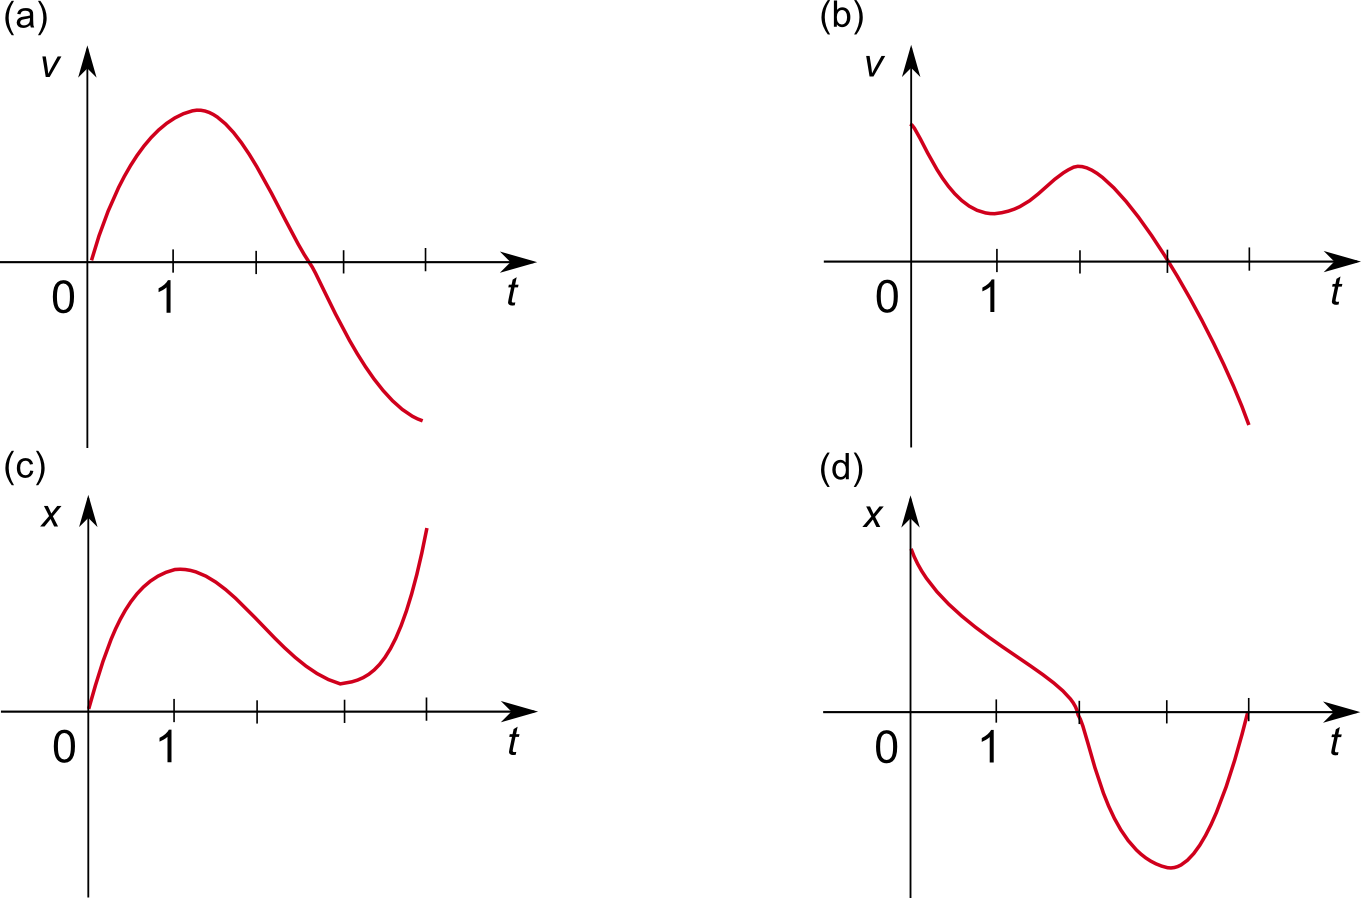
\includegraphics[width=0.6\textwidth]{matematik/vx_grafer.png}
  \caption{Hastighed og position som funktion af tiden.}
  \label{fig:vx_grafer}
\end{figure}
\opg Da grafen simpelt viser $v$ som funktion af tiden kan man bare aflæse på figuren.
for (a): 
\begin{itemize}
\item $t= 0 \rightarrow 1,5$: sætter farten op
\item $t= 1,5 \rightarrow 4$: sætter farten ned
\end{itemize}
for (b):
\begin{itemize}
\item $t= 0 \rightarrow 1$: sætter farten ned
\item $t= 1 \rightarrow 2$: sætter farten op
\item $t= 2 \rightarrow 4$: sætter farten ned
\end{itemize}
.
\opg Her ses i stedet positionen som funktion af tiden. For at svare på, hvordan hastigheden opfører sig, så skal vi derfor kigge på \emph{hældningen} af grafen.
for (c): 
\begin{itemize}
\item $t= 0 \rightarrow 1$: positiv hældning $\rightarrow$ hastigheden øges
\item $t= 1 \rightarrow 3$: negativ hældning $\rightarrow$ hastigheden sænkes
\item $t= 3 \rightarrow 4$: positiv hældning $\rightarrow$ hastigheden øges
\end{itemize}
for (d):
\begin{itemize}
\item $t= 0 \rightarrow 2$: negativ hældning $\rightarrow$ hastigheden sænkes
\item $t= 2 \rightarrow 3$: negativ hældning $\rightarrow$ hastigheden sænkes - og hældningen er større, så der bremses hårdere.
\item $t= 3 \rightarrow 4$: positiv hældning $\rightarrow$ hastigheden øges
\end{itemize}
.
\end{opgave}
\begin{opgave}{Harmonisk bevægelse}{2}
\begin{equation*}
x = A \cos (\omega t + \phi),
\end{equation*}
hvor $A$, $\omega$ og $\phi$ er konstanter. 
\opg For at finde hastigheden ($\dt{x}$), så ses det at udtrykket er en sammensat funktion ($g=\omega t+\phi$, $f=A\cos g$). Bruges kædereglen får man:
\begin{equation*}
\dt{x} = - A\omega \sin(\omega t + \phi)
\end{equation*}
\opg Hvis det antages at alle konstanter er $>0$, så er $\dt{x}=0$, når $\sin(\omega t + \phi) = 0$. Det er opfyldt for $\omega t + \phi = 0, \pi, 2\pi, ...$. Fysisk set er $v=0$ i yderpunkterne af svingningen, som forekommer periodisk.
\end{opgave}
\begin{opgave}{Cepheide-stjernen Delta Cephei}{2}
\begin{equation*}
B(t) = 4,0 + 0,35\sin \left( \frac{2\pi t}{5,4} \right).
\end{equation*}
\opg Raten er $\d{B}{t} = \dt{B}$. Funktionen er en sammensat funktion ($u=\frac{2\pi t}{5,4}, g=0,4+0,35 \sin u$).
\begin{equation*}
\dt{B} = 0,35 \cdot \frac{2\pi}{5,4} \cos \left( \frac{2\pi t}{5,4} \right)
\end{equation*}
\opg For at finde ændringen i lysstyrke udregnes forskellen:
\begin{align*}
B(t=\text{2 dage})-B(t=\text{0 dage}) \\
&= 4,0 + 0,35\sin\left(\frac{2\pi}{5,4} \cdot 2 \right) - 4,0 -0,35\sin\left(\frac{2\pi}{5,4} \cdot 0 \right) \\
&= 0,25
\end{align*}
Husk at regne i radianer og ikke i grader.
\end{opgave}

\begin{opgave}{Udvidelse af ballon}{2}
\opg $\d{V}{r}$ er ændring af volumen afhængig af radius, mens $\d{V}{t}$ er ændring af volumen afhængig af tiden.
\opg Volumenet af en sfærisk ballon er $V(t)=\frac{4}{3} \pi r(t)^3$. Det er en sammensat funktion med $u=r(t)$ og $g=\frac{4}{3} \pi u^3$. Det giver:
\begin{equation*}
\dt{V} = \frac{4}{3} 2\pi \cdot 3 r^2(t) \dt{r}
\end{equation*}
\end{opgave}

\begin{opgave}{Approksimation af funktion}{3}
  \[
  f(x) = f(a) + (x-a) \left.\d{f}{x}\right|_{x=a}
  + \tfrac{1}{2} (x-a)^2 \left.\dd{f}{x}\right|_{x=a}
  + \tfrac{1}{3!} (x-a)^3 \left.\frac{d^3f}{dx^3}\right|_{x=a}
  + \ldots
  \]
  \opg Første led er en konstant, mens andet led afhænger linært af $x$, og tredje led kvadratisk af $x$ osv. Forfaktoren bliver mindre og mindre for hvert led, så ledene bliver mindre og mindre.
  \opg For $x \approx 0$, er $\sin x$ med de første to led:
  \begin{align*}
  \sin x &= \sin(0) + (x-0) \left. \d{\sin x}{x}\right|_{x=0} \\
  &= 0 + x\cos(0) \\
  &= x
  \end{align*}
  Idet $\sin(0)=0$ og $\cos(0)=1$.
  For $x \approx 0$, er $\cos x$ med de første to led:
  \begin{align*}
  \cos x &= \cos(0) + (x-0) \left.\d{\sin x}{x}\right|_{x=0} \\
  &= 1 -x\sin(0) \\
  &= 1
  \end{align*}
  Hvis man medtager det 3. led, så bliver $\sin(x)$:
  \begin{align*}
  \sin(x) &= x + \frac{1}{2} (x-0)^2 \left. \dd{\sin(x)}{x}\right|_{x=0} \\
  &= x - \frac{x^2}{2} \sin(0) \\
  &= x  
  \end{align*}
  Hvis man medtager det 3. led, så bliver $\cos(x)$:
  \begin{align*}
  \cos(x) &= 1 + \frac{1}{2} (x-0)^2 \left.\dd{\cos(x)}{x}\right|_{x=0} \\
  &= 1 - \frac{x^2}{2} \cos(0) \\
  &= 1 - \frac{x^2}{2}  
  \end{align*}
  \opg For $x \approx 1$, er $\ln x$ for de tre første to led:
  \begin{align*}
  \ln x &= \ln(1) + (x-1) \left. \d{\ln x}{x} \right|_{x=1} + \frac{1}{2} \left(x-1\right)^2 \left. \dd{\ln x}{x}\right|_{x=1} \\
  &= 0 + (x-1)\frac{1}{1} - \frac{1}{2} \left( x^2 +1 - 2x \right) \left. \d{}{x} \frac{1}{x} \right|_{x=1} \\
  &= x -1 + \frac{1}{2} \left( x^2 + 1 - 2x \right) \left. \left( -1 x^{-2} \right)\right|_{x=1} \\
  &= x - 1 - \frac{x^2}{2} - \frac{1}{2} + x\\
  &= - \frac{x^2}{2} + 2x - \frac{3}{2}
  \end{align*}
  Idet den differentierede at $\ln x = \frac{1}{x}$ og $\ln 1=0$.
  \opg For $x \approx 0$, er $e^x \approx 1 + x + \frac{1}{2}
  x^2$ for de første tre led:
  \begin{align*}
  e^x &= e^0 + (x-0) \left. \d{e^x}{x}\right|_{x=0} + \frac{1}{2}(x-0)^2 \left. \dd{e^x}{x}\right|_{x=0} \\
  &=1 + x + \frac{1}{2} x^2,
  \end{align*}
  Idet den differentierede af $e^x$ er $e^x$ og $e^0 = 1$.
  \opg For $x \approx 0$, vises det, at approksimationen for et polynomie
  $a_0 + a_1 x + a_2 x^2 + \ldots$ er givet ved leddene i polynomiet
  selv. Vi regner ét led af gangen:
  \begin{align*}
  \text{Første led } &= a_0 + a_1\cdot 0 + a_2 \cdot 0^2 \\
  &= a_0 \\
  \text{Andet led } &= (x-0) \left. \d{}{x} \left(a_0 + a_1x + a_2x^2 \right)\right|_{x=0} \\
  &= x \cdot \left. \left(a_1 + 2a_2x) \right)\right|_{x=0} \\
  &= a_1 x \\
  \text{Tredje led} &= \frac{1}{2} \left( x-0 \right)^2 \left. \dd{}{x} \left(a_0 + a_1x + a_2x^2 \right)\right|_{x=0} \\
  &= \frac{1}{2} x^2 \left. \d{}{x} \left(a_1 + 2a_2x \right)\right|_{x=0} \\
  &= \frac{1}{2} x^2 \left. \left( 2a_2 \right)\right|_{x=0} \\
  &= a_2 x^2 \\
  \rightarrow & a_0 + a_1x+a_2x^2
  \end{align*}
  Og det er hermed vist at approksimationen af et polynomie er givet ved leddene i polynomiet.
  \opg For små værdier af $x$ ($x \approx 0$), vises det, at $(1 + x)^a \approx 1 + ax$.:
  \begin{align*}
  (1+x)^a &= (1+0)^a + (x-0) \left. \d{(1+x)^a}{x}\right|_{x=0} \\
  &= 1 + \left. \left( a(1+x)^{a-1} \right)\right|_{x=0} \\
  &= 1 + ax,
  \end{align*}
  hvor $(1+x)^a$ er blevet differentieret som en sammensat funktion med $u=1+x$ og $g=u^a$.
\end{opgave}

\newpage

\section*{Differentialligninger}

\begin{opgave}{Specialtilfælde af 1. og 2. Ordens Differentialligninger}{1}
\opg $f(t) = -7e^{3t}$ og $\d{f}{t} = 3f(t)$.

$$\d{f}{x} = -7 \dl{e^{3t}}{t} = -7 \cdot 3 e^{3t} = 3 \left( -7 e^{3t} \right) = 3 f(t)$$
\vspace{2mm}
\opg $g(t) = \frac{2}{3}e^t + e^{-2t}$ og $\d{g}{t} + 2g(t) = 2e^t$.

$$\d{g}{t} = \frac{2}{3} \dl{e^t}{t} + \dl{e^{-2t}}{t} = \frac{2}{3}e^t -2e^{-2t} \quad \Rightarrow \quad \d{g}{t} + 2g(t) = \frac{2}{3}e^t -2e^{-2t} + \frac{4}{3}e^t + 2e^{-2t} = \frac{6}{3} e^t = 2e^t$$
\vspace{2mm}
\opg $h(t) = 5 \sin(3t) - 10\cos(3t)$ og $\dd{h}{t} = -9h(t)$.

$$\d{h}{t} = 3 \cdot 5 \cos(3t) + 3 \cdot 10 \sin(3t) \quad \Rightarrow \quad \dd{h}{t} = (-9) \cdot 5 \cos(3t) + 9 \cdot 10 \sin(3t) = -9 h(t)$$
\vspace{2mm}
\opg $k(t) = 13 \cos \left( 8t + 45 \right)$ og $\dd{k}{t} = -64 k(t)$.

$$\d{k}{t} = (-8) \cdot 13 \cos \left( 8t + 45 \right) \quad \Rightarrow \quad \dd{k}{t} = (-64) \cdot 13 \cos \left( 8t + 45 \right) = -64 k(t)$$
\vspace{2mm}
\end{opgave}

\begin{opgave}{Generelle 1. Ordens Differentialligninger}{2}
\opg $h(x) = 1/ \left( x+A \right)$ og $\d{h}{x} = -h(x)^2$.

$$\d{h}{x} = \dl{\left( x+A \right)^{-1}}{x} = - \left( x+A \right)^{-2} \dl{\left( x+A \right)}{x} = - \frac{1}{\left( x + A \right)^2} = -h(x)^2$$
\vspace{2mm}
\opg $k(x) = \left( c-x^2 \right)^{-1/2}$ og $\d{k}{x} = x k(x)^3$.

$$\d{k}{x} = - \frac{1}{2} \left( c-x^2 \right)^{-3/2}  \dl{\left( c-x^2 \right)}{x} = x \left( c-x^2 \right)^{-3/2} = x k(x)^3$$
\vspace{2mm}
\opg $g(x) = \left( \ln x + C \right)/x$ og $x^2 \d{g}{x} + x g(x) = 1$.

$$\d{g}{x} = \left[ \dl{\left( \ln x + C \right)}{x} \right] \frac{1}{x} + \left( \ln x + C \right)  \left[ \dl{\frac{1}{x}}{x} \right]  = \frac{1}{x^2} - \frac{\ln x + C}{x^2} \quad \Rightarrow \quad x^2 \d{g}{x} + xg(x) = 1 - \left( \ln x + C \right) + \left( \ln x + C \right) = 1$$
\vspace{2mm}
\opg $f(x) = \left( 1+ce^x \right)/\left( 1-ce^x \right)$ og $\d{f}{x} = \frac{1}{2} \left( f(x)^2 -1 \right)$.

\begin{align*}
\d{f}{x} &= \left[ \dl{\left( 1+c^x \right)}{x} \right] \frac{1}{1-ce^x} + \left( 1+ce^x \right) \left[ \dl{\frac{1}{1-ce^x}}{x} \right] = \frac{ce^x}{1-ce^x} +  \frac{\left( 1+ce^x \right) \left( -1 \right) \left( -ce^x \right)}{\left( 1-ce^x \right)^2}\\\\
&= ce^x \left[ \frac{1}{1-ce^x} + \frac{1+ce^x}{\left( 1-ce^x \right)^2} \right] = ce^x \frac{1-ce^x + 1+ce^x}{\left( 1-ce^x \right)^2} = \frac{2ce^x}{\left( 1-ce^x \right)^2}
\end{align*}

$$f(x)^2 - 1  =  \frac{\left( 1+ce^x \right)^2}{\left( 1-ce^x \right)^2} - \frac{(1-ce^x)^2}{\left( 1-ce^x \right)^2} = \frac{\left( 1+ce^x \right)^2 - \left( 1-ce^x \right)^2}{\left( 1-ce^x \right)^2} = \frac{4ce^x}{\left( 1-ce^x \right)^2} \quad \Rightarrow \quad \d{f}{x} = \frac{1}{2} \left( f(x)^2 -1 \right)$$
\end{opgave}

\begin{opgave}{Hvornår er det en løsning?}{3}
\opg Find $k$ så $f(y) = \cos(ky)$ løser $4 \dd{f}{y} = -25f(y)$.

$$\d{f}{y} = -k\sin(ky) \quad \Rightarrow \quad \dd{f}{y} = -k^2 \cos(ky) = -k^2 f(y)$$

\vspace{2mm}

Så sætter man ind:

$$4 \dd{f}{y} = -25f(y) \quad \Rightarrow \quad -4k^2 f(y) = -25f(y) \quad \Rightarrow \quad k^2 = \frac{25}{4} \quad \Rightarrow \quad k = \pm \frac{5}{2}$$
\vspace{2mm}
\opg For de fundne $k$ fra 1), vis at $g(y) = A\sin(ky) + B\cos(ky)$ løser $4 \dd{g}{y} = -25g(y)$.

$$\d{g}{y} = kA\cos(ky) - kB\sin(ky) \quad \Rightarrow \quad \dd{g}{y} = -k^2 A \sin(ky) - k^2 B \cos(ky) = -k^2g(y)$$

\vspace{2mm}

Det giver:

$$-4k^2 g(y) = -25g(y) $$

\vspace{2mm}

Som er opfyldt for $k = \pm \frac{5}{2}$.\\
\opg Find $r$ så $h(y) = e^{ry}$ løser $2 \dd{h}{y} + \d{h}{y} - h(y) = 0$.

$$\d{h}{y} = re^{ry} = rh(y) \quad \Rightarrow \quad \dd{h}{y} = r^2 e^{ry} = r^2 h(y)$$

\vspace{2mm}

Så sætter man ind:

$$2 \dd{h}{y} + \d{h}{y} - h(y) = 0 \quad \Rightarrow \quad 2r^2h(y) + rh(y) -h(y) = 0 \quad \Rightarrow \quad 2r^2+r-1=0$$
\vspace{2mm}

Løses andengradsligningen får man:

$$r_1 = \frac{1}{2} \quad \text{og} \quad r_2 = -1$$ 
\vspace{2mm}
\opg For de fundne $r_1,r_2$ i 3), vis at $k(y) = ae^{r_1y} + be^{r_2y}$ løser $2 \dd{k}{y} + \d{k}{y} - k(y) = 0$.

$$\d{k}{y} = ar_1e^{r_1y} + br_2e^{r_2y} \quad \Rightarrow \quad \dd{k}{y} = ar_1^2e^{r_1y} + br_2^2e^{r_2y}$$ 
\vspace{2mm}

Så sætter man ind:

\begin{align*}
2 \dd{k}{y} + \d{k}{y} - k(y) &= 2 \left( ar_1^2e^{r_1y} + br_2^2e^{r_2y}  \right) + \left( ar_1e^{r_1y} + br_2e^{r_2y} \right) - \left( ae^{r_1y} + be^{r_2y} \right)\\\\ 
&= \left( 2ar_1^2 + ar_1 - a \right)e^{r_1y} + \left( 2br_2^2 + br_2 - b \right)e^{r_2y} = 0 \cdot e^{r_1y} + 0 \cdot e^{r_2y} = 0 
\end{align*}
\end{opgave}



